\begin{align}
    \vec{V}=\vec{V}^T=\myvec{a & b \\ b & c}=\myvec{12 & \frac{k}{2} \\ \frac{k}{2} & 2}\label{eq:solutions/13/8/2.3}\\
    \vec{u}=\myvec{d \\ e}=\myvec{\frac{11}{2} \\ -\frac{5}{2}}\label{eq:solutions/13/8/2.4}
\end{align}

The equation \eqref{eq:solutions/13/8/1.1} represents pair of straight lines if
\begin{align}
    &\mydet{\vec{V} & \vec{u} \\ \vec{u}^T & f}=0\\
    \implies&\mydet{12 & \frac{k}{2} & \frac{11}{2} \\ \frac{k}{2} & 2 & -\frac{5}{2} \\ \frac{11}{2} & -\frac{5}{2} & 2}=0\label{eq:solutions/13/8/2.6}\\
    \implies&\mydet{24 & k & 11 \\ k & 4 & -5 \\ 11 & -5 & 4}=0\\
    \implies&24\mydet{ 4 & -5 \\ -5 & 4}-k\mydet{ k & -5 \\ 11 & 4}+11\mydet{ k & 4 \\ 11 & -5}=0
\end{align}
\begin{align}
    \implies2k^2+55k+350=0\\
    \implies(10+k)(2k+35)=0\\
    \implies k=-10\nonumber\\
    k=-\frac{35}{2}
\end{align}
Therefore, for $k=-10$ and $k=-\frac{35}{2}$ the given equation represents pair of straight lines.\\
Now Lets find equation of lines for $k=-10$.
\noindent
Substitute $k=-10$ in \eqref{eq:solutions/13/8/1.1}. We get equation of pair of straight lines as:
\begin{align}
    12x^2-10xy+2y^2+11x-5y+2=0
\end{align}
%Comparing above equation with \eqref{eq:solutions/13/8/2.1}, we will get $a=12$, $b=-5$, $c=2$, $d=\frac{11}{2}$, $e=-\frac{5}{2}$, $f=2$.\\
From \eqref{eq:solutions/13/8/1.1}, \eqref{eq:solutions/13/8/2.3}, \eqref{eq:solutions/13/8/2.4} we get
\begin{align}
    \vec{V}=\vec{V}^T=\myvec{12 & -5 \\ -5 & 2}\label{eq:solutions/13/8/2.17}\\
    \vec{u}=\myvec{\frac{11}{2} \\ -\frac{5}{2}}\label{eq:solutions/13/8/2.18}
\end{align}
\noindent
If $\mydet{\vec{V}}<0$ then two lines will intersect.
\begin{align}
    \mydet{\vec{V}}&=\mydet{12 & -5 \\ -5 & 2}\\
    \implies\mydet{\vec{V}}&=-1\\
    \implies\mydet{\vec{V}}&<0
\end{align}
\noindent
Therefore the lines will intersect.\\
The equation of two lines is given by
\begin{align}
    \vec{n_1}^T\vec{x}=c_1\label{eq:solutions/13/8/1.12}\\
    \vec{n_2}^T\vec{x}=c_2\label{eq:solutions/13/8/1.13}
\end{align}
Equating their product with \eqref{eq:solutions/13/8/1.1}
\begin{multline}
    (\vec{n_1}^T\vec{x}-c_1)(\vec{n_2}^T\vec{x}-c_2)\\=\vec{x}^T\vec{V}\vec{x}+2\vec{u}^T\vec{x}+f=0
\end{multline}
\begin{align}
    \implies\vec{n_1}*\vec{n_2}&=\myvec{a \\ 2b \\c}=\myvec{12\\-10\\2}\label{eq:solutions/13/8/conv}
\end{align}
\begin{align}
    c_2\vec{n_1}+c_1\vec{n_2}&=-2\vec{u}=-2\myvec{\frac{11}{2} \\ -\frac{5}{2}}\label{eq:solutions/13/8/1.16}\\
    c_1c_2&=f=2
\end{align}
The slopes of the lines are given by roots of equation
\begin{align}
    cm^2+2bm+a=0\label{eq:solutions/13/8/poly}\\
    \implies 2m^2-10m+12=0\\
    m_i=\frac{-b\pm{\sqrt{-\mydet{\vec{V}}}}}{c}\\
    \implies m_i=\frac{5\pm{\sqrt{1}}}{2}\\
    \implies m_1=3\\
     m_2=2
\end{align}
The normal vector for two lines is given by
\begin{align}
    \vec{n_i}=k_i\myvec{-m_i\\1}\label{eq:solutions/13/8/normvec}\\
    \implies\vec{n_1}=k_1\myvec{-3\\1}\label{eq:solutions/13/8/n1}\\
    \vec{n_2}=k_2\myvec{-2\\1}\label{eq:solutions/13/8/n2}
\end{align}
Substituting \eqref{eq:solutions/13/8/n1},\eqref{eq:solutions/13/8/n2} in \eqref{eq:solutions/13/8/conv}. we get
\begin{align}
    k_1k_2=2
\end{align}
The possible combinations of ($k_1$,$k_2$) are (1,2), (2,1), (-1,-2) and (-2,-1).\\
lets assume $k_1=1$,$k_2=2$ we get
\begin{align}
    \implies\vec{n_1}=\myvec{-3\\1}\label{soln1}\\
    \vec{n_2}=\myvec{-4\\2}\label{soln2}
\end{align}
We verify obtained $\vec{n_1}$,$\vec{n_2}$ using Toeplitz matrix
\begin{align}
    \vec{n_1}*\vec{n_2}=\myvec{-3 & 0\\1 & -3\\0 & 1}\myvec{-4 \\ 2}=\myvec{12\\-10\\2}\label{eq:solutions/13/8/comp1}\\
    \implies \vec{n_1}*\vec{n_2}=\myvec{12\\-10\\2}=\myvec{a\\2b\\c}
\end{align}
Therefore the obtained $\vec{n_1}$,$\vec{n_2}$ are correct.\\
Substitute \eqref{soln1}, \eqref{soln2} in \eqref{eq:solutions/13/8/1.16}
and calculate for $c_1$ and $c_2$

\begin{align}
    c_2\myvec{-3\\1}+c_1\myvec{-4\\2}=\myvec{ -11\\ -5}
\end{align}
Solve using row reduction technique.
\begin{align}
    \implies\myvec{-4 & -3 & -11\\2 & 1 & -5}\\
    \xleftrightarrow[]{R_2\leftarrow 2R_2+R_1}\myvec{-4 & -3 & -11\\0 & -1 & -21}\\
    \xleftrightarrow[]{R_1\leftarrow R_1-3R_2}\myvec{-4 & 0 & 52\\0 & -1 & -21}\\
    \implies\myvec{1 & 0 & -13\\0 & 1 & 21}\\
    \implies c_1=-13\label{c1}\\
    c_2=21\label{c2}
\end{align}

Substituting \eqref{soln1},\eqref{soln2},\eqref{c1},\eqref{c2} in \eqref{eq:solutions/13/8/1.12} and \eqref{eq:solutions/13/8/1.13}. We get equation of two straight lines.
\begin{align}
    \myvec{-3 & 1}\vec{x}=-13\\
    \myvec{-4 & 2}\vec{x}=21
\end{align}

The plot of these two lines is shown in Fig.~\ref{fig:solutions/13/8/figure1}.
\begin{figure}[ht!]
    \centering
    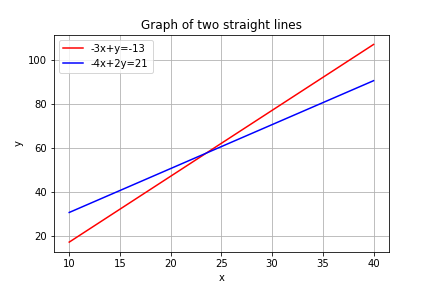
\includegraphics[width=\columnwidth]{./solutions/13/8/Figure1}
    \caption{Pair of straight lines for $k=-10$}
    \label{fig:solutions/13/8/figure1}
\end{figure}

Now Lets find equation of lines for $k=-\frac{35}{2}$.

Substitute $k=-\frac{35}{2}$ in \eqref{eq:solutions/13/8/1.1}. We get equation of pair of straight lines as:
\begin{align}
    12x^2-\frac{35}{2}xy+2y^2+11x-5y+2=0
\end{align}

%Comparing above equation with \eqref{eq:solutions/13/8/2.1}, we will get $a=12$, $b=-\frac{35}{4}$, $c=2$, $d=\frac{11}{2}$, $e=-\frac{5}{2}$, $f=2$.\\
From \eqref{eq:solutions/13/8/1.1}, \eqref{eq:solutions/13/8/2.3}, \eqref{eq:solutions/13/8/2.4} we get
\begin{align}
    \vec{V}=\vec{V}^T=\myvec{12 & -\frac{35}{4} \\ -\frac{35}{4} & 2}\label{eq:solutions/13/8/2.48}\\
    \vec{u}=\myvec{\frac{11}{2} \\ -\frac{5}{2}}\label{eq:solutions/13/8/2.49}
\end{align}
If $\mydet{\vec{V}}<0$ then two lines will intersect.
\begin{align}
    \mydet{\vec{V}}&=\mydet{12 & -\frac{35}{4} \\ -\frac{35}{4} & 2}\\
    \implies\mydet{\vec{V}}&=-\frac{841}{16}\\
    \implies\mydet{\vec{V}}&<0
\end{align}
Therefore the lines will intersect.\\
Now from \eqref{eq:solutions/13/8/conv},
\begin{align}
    \implies\vec{n_1}*\vec{n_2}&=\myvec{a \\ 2b \\c}=\myvec{12\\-\frac{35}{2}\\2}\label{eq:solutions/13/8/conv2}
\end{align}
The slopes of the lines are given by roots of equation \eqref{eq:solutions/13/8/poly}
\begin{align}
    \implies 2m^2-\frac{35}{2}m+12=0\\
    m_i=\frac{-b\pm{\sqrt{-\mydet{\vec{V}}}}}{c}\\
    \implies m_i=\frac{\frac{35}{4}\pm{\sqrt{\frac{841}{16}}}}{2}\\
    \implies m_1=8\\
     m_2=\frac{3}{4}
\end{align}
The normal vector for two lines is given by \eqref{eq:solutions/13/8/normvec}
\begin{align}
    \implies\vec{n_1}=k_1\myvec{-8\\1}\label{eq:solutions/13/8/n3}\\
    \vec{n_2}=k_2\myvec{-\frac{3}{4}\\1}\label{eq:solutions/13/8/n4}
\end{align}
Substituting \eqref{eq:solutions/13/8/n3},\eqref{eq:solutions/13/8/n4} in \eqref{eq:solutions/13/8/conv2}. we get
\begin{align}
    k_1k_2=2
\end{align}
The possible combinations of ($k_1$,$k_2$) are (1,2), (2,1), (-1,-2) and (-2,-1).\\
lets assume $k_1=1$,$k_2=2$ we get

\begin{align}
    \implies\vec{n_1}=\myvec{-8\\1}\label{soln3}\\
    \vec{n_2}=\myvec{-\frac{3}{2}\\2}\label{soln4}
\end{align}
We verify obtained $\vec{n_1}$,$\vec{n_2}$ using Toeplitz matrix
\begin{align}
    \vec{n_1}*\vec{n_2}=\myvec{-8 & 0\\1 & -8\\0 & 1}\myvec{-\frac{3}{2} \\ 2}=\myvec{12\\-\frac{35}{2}\\2}\\
    \implies\vec{n_1}*\vec{n_2}=\myvec{12\\-\frac{35}{2}\\2}=\myvec{a\\ 2b \\ c}
\end{align}
Therefore the obtained $\vec{n_1}$,$\vec{n_2}$ are correct.\\
Substitute \eqref{soln3}, \eqref{soln4} in \eqref{eq:solutions/13/8/1.16} we get 
\begin{align}
    c_2\myvec{-8\\1}+c_1\myvec{-\frac{3}{2}\\2}=\myvec{ -11\\ -5}
\end{align}
Solve using row reduction technique.
\begin{align}
    \implies\myvec{-\frac{3}{2} & -8 & -11\\2 & 1 & -5}\\
    \xleftrightarrow[]{R_1\leftarrow 2R_1}\myvec{-3 & -16 & -22\\2 & 1 & -5}\\
    \xleftrightarrow[]{R_2\leftarrow 3R_2+2R_1}\myvec{-3 & -16 & -22\\0 & -29 & -59}\\
    \xleftrightarrow[]{R_1\leftarrow 29R_1-16R_2}\myvec{-87 & 0 & 306\\0 & -29 & -59}\\
    \implies\myvec{1 & 0 & -\frac{102}{29}\\0 & 1 & \frac{59}{29}}\\
    \implies c_1=-\frac{102}{29}\label{c3}\\
    c_2=\frac{59}{29}\label{c4}
\end{align}

Substituting \eqref{soln3},\eqref{soln4},\eqref{c3},\eqref{c4} in \eqref{eq:solutions/13/8/1.12} and \eqref{eq:solutions/13/8/1.13}. we get equation of two straight lines.
\begin{align}
    \myvec{-8 & 1}\vec{x}=-\frac{102}{29}\\
    \myvec{-\frac{3}{2} & 2}\vec{x}=\frac{59}{29}
\end{align}
%\newpage
%The plot of these two lines is shown in Fig.~\ref{fig:solutions/13/8/figure2}.
%\begin{figure}[ht!]
%    \centering
%    \includegraphics[width=\columnwidth]{./solutions/13/8/Figure2}
%    \caption{Pair of straight lines for $k=-\frac{35}{2}$}
%    \label{fig:solutions/13/8/figure2}
%\end{figure}
